%%%%%%%%%%%%%%%%%%%%%%%%%%%%%%%%%%%%%%%%%
% Quiz #1 Template
% LaTeX Template
% By: Ryan Grove
%%%%%%%%%%%%%%%%%%%%%%%%%%%%%%%%%%%%%%%%%

%----------------------------------------------------------------------------------------
%	PACKAGES AND OTHER DOCUMENT CONFIGURATIONS
%----------------------------------------------------------------------------------------

\documentclass[paper=a4, fontsize=11pt]{scrartcl} % A4 paper and 11pt font size

\usepackage[T1]{fontenc} % Use 8-bit encoding that has 256 glyphs
\usepackage{fourier} % Use the Adobe Utopia font for the document - comment this line to return to the LaTeX default
\usepackage[english]{babel} % English language/hyphenation
\usepackage{amsmath,amsfonts,amsthm} % Math packages

\usepackage{lipsum} % Used for inserting dummy 'Lorem ipsum' text into the template

\usepackage{sectsty} % Allows customizing section commands
\allsectionsfont{\centering \normalfont\scshape} % Make all sections centered, the default font and small caps

\usepackage{fancyhdr} % Custom headers and footers
\pagestyle{fancyplain} % Makes all pages in the document conform to the custom headers and footers
\fancyhead{} % No page header - if you want one, create it in the same way as the footers below
\fancyfoot[L]{} % Empty left footer
\fancyfoot[C]{} % Empty center footer
%\fancyfoot[R]{\thepage} % Page numbering for right footer
\renewcommand{\headrulewidth}{0pt} % Remove header underlines
\renewcommand{\footrulewidth}{0pt} % Remove footer underlines
\setlength{\headheight}{13.6pt} % Customize the height of the header

\numberwithin{equation}{section} % Number equations within sections (i.e. 1.1, 1.2, 2.1, 2.2 instead of 1, 2, 3, 4)
\numberwithin{figure}{section} % Number figures within sections (i.e. 1.1, 1.2, 2.1, 2.2 instead of 1, 2, 3, 4)
\numberwithin{table}{section} % Number tables within sections (i.e. 1.1, 1.2, 2.1, 2.2 instead of 1, 2, 3, 4)

\setlength\parindent{0pt} % Removes all indentation from paragraphs - comment this line for an assignment with lots of text

\usepackage{lastpage}
\usepackage{fancyhdr}
\cfoot{\thepage\ of \pageref{LastPage}}

\def\v{\hbox{$\mathbf v$}}
\def\w{\hbox{$\mathbf w$}}
\def\u{\hbox{$\mathbf u$}}
\def\x{\hbox{$\textbf{x}$}}
\def\z{\hbox{$\mathbf z$}}
\def\a{\hbox{$\mathbf a$}}
\def\b{\hbox{$\mathbf b$}}
\def\L{\hbox{$\mathcal L$}}
\def\C{\hbox{$\mathbb C$}}
\def\B{\hbox{$\mathcal B$}}
\def\R{\hbox{$\mathbb R$}}
\def\X{\hbox{$\underline X$}}
\def\Q{\hbox{$\mathbb Q$}}
\def\R{\hbox{$\mathbb R$}}
\def\N{\hbox{$\mathbb N$}}
\def\C{\hbox{$\mathbb C$}}
\def\0{\hbox{$\mathbf 0$}}
\def\Y{\hbox{$\underline Y$}}
\def\a{\hbox{$\mathbf a$}}
\def\u{\hbox{$\mathbf u$}}
\def\w{\hbox{$\mathbf w$}}
\def\y{\hbox{$\mathbf y$}}
\def\X{\hbox{$\underline X$}}
\def\dd{\hbox{$\partial $}}
\def\B{\hbox{$\mathcal B$}}
\def\F{\hbox{$\mathcal F$}}
\def\L{\hbox{$\mathcal L$}}
\def\M{\hbox{$\mathcal M$}}
\def\D{\hbox{$\mathscr {D}$}}
\def\RR{\hbox{$\mathscr{R}$}}
\def\I{\hbox{$\mathcal I$}}

\usepackage{amssymb}
%\theoremstyle{plain}
\usepackage[margin = .75in]{geometry}
\newtheorem{claim}{Claim}
\newtheorem{theorem}{Theorem}[section]
\newtheorem{lemma}[theorem]{Lemma}
\newtheorem{proposition}[theorem]{Proposition}
\newtheorem{corollary}[theorem]{Corollary}
\newtheorem{problem}[theorem]{Problem}
%\theoremstyle{definition}
\newtheorem{definition}[theorem]{Definition}
%\theoremstyle{remark}
\newtheorem{remark}[theorem]{Remark}
\newtheorem{remarks}[theorem]{Remarks}
\newtheorem{example}[theorem]{Example}
\newcommand{\ds}{\displaystyle}
\newcommand{\ZZ}{\mathbb{Z}}
\newcommand{\QQ}{\mathbb{Q}}
\newcommand{\e}{\varepsilon}
\newcommand{\bbf}{\textbf}
\newcommand{\p}{\parallel}
\usepackage{color}
\newcommand{\field}[1]{\mathbb{#1}}
\usepackage{amsmath}
\usepackage{amsthm}
\usepackage{amssymb}
\usepackage{mathrsfs}
\usepackage{cancel}
\usepackage{upgreek}
\usepackage{graphicx}
\usepackage{multirow}
\usepackage{setspace}
\usepackage{url}
\usepackage{subfigure}
\usepackage{enumerate}
\usepackage{cases}
\usepackage{mathrsfs}
\usepackage{rotating}

%----------------------------------------------------------------------------------------
%	TITLE SECTION
%----------------------------------------------------------------------------------------

\newcommand{\horrule}[1]{\rule{\linewidth}{#1}} % Create horizontal rule command with 1 argument of height

\title{	
\normalfont \normalsize 
\textsc{Ryan Grove, Clemson University, MATH1080 - 9} \\ [25pt] % Your name, university, class
\horrule{0.5pt} \\[0.4cm] % Thin top horizontal rule
\huge Section 6.2: Volumes \\ % The assignment title
\horrule{2pt} \\[0.5cm] % Thick bottom horizontal rule
}

\author{Date:} % The due date

\date{\normalsize January 12, 2016} % A custom date

\begin{document}

\maketitle % Print the title

\begin{flushleft}
\begin{tabular}{l l}
Name: \rule{3.2in}{.01cm}  & {}%Table number: \rule{1in}{.01cm}\\
\end{tabular}
\end{flushleft}

%----------------------------------------------------------------------------------------
%	Lecture
%----------------------------------------------------------------------------------------

\section*{\textbf{Lecture:}}

\section*{Using Cross-Sections to Find Volume}
To find the volume of a solid $S$ (that isn't a well-known shape) we start by intersecting $S$ with a plane and obtaining a plane region that is called a \underline{\hspace{1.5in}} of $S$. Let \underline{\hspace{0.5in}} be the area of the cross-section of $S$ in a plane $P_x$ perpendicular to the $x$-axis and passing through the point $x$, where $a\leq x \leq b$. (See Figure 2 below. Think of slicing $S$ with a knife through $x$ and computing the area of this slice.) The cross-sectional area $A(x)$ will vary as $x$ increases from $a$ to $b$.\\

\[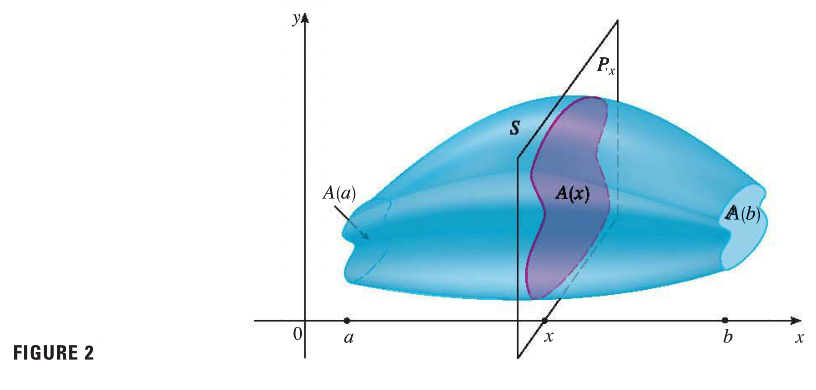
\includegraphics[scale=0.38]{6-2pic1.png}\]

Let's divide $S$ into $n$ "slabs" of equal width $\Delta x$ to slice the solid. (Think of slicing a loaf of bread.)

\[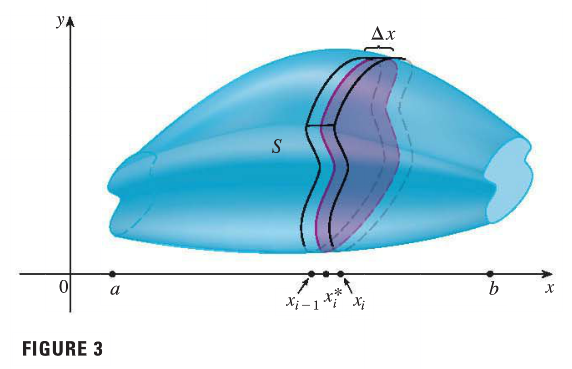
\includegraphics[scale=0.38]{6-2pic2.png}\]

The volume of the $i^{\text{th}}$ slab is\\

\[\underline{\hspace{1.5in}}\]
where $A(x_i^*)$ is the area of the base of the slab and $\Delta x$ is the width. (Like volume of a cylinder). \\
\indent

Adding the volumes of these slabs, we get an approximation to the total volume:\\

\[\underline{\hspace{1.5in}}\]

This approximation becomes better and better as \underline{\hspace{0.75in}}. (Think of the slices as becoming thinner and thinner.) Therefore we define the volume as the limit of these sums as $n\to\infty$. But we recognize the limit of Riemann sums as a \underline{\hspace{1in}} \underline{\hspace{1in}} and so we have the following definition.\\
\indent


\fbox{
  \parbox{\textwidth}{
  \vspace{5pt} \textbf{Definition of Volume:} Let $S$ be a solid that lies between $x=a$ and $x=b$. If the cross-sectional area of $S$ in the plane $P_x$, through $x$ and perpendicular to the $x-$axis, is $A(x)$, where $A$ is a continuous function, then the \underline{\textbf{volume}} of $S$ is:\\
  
  \[\underline{\hspace{2.25in}}\]
  \indent
  
  }}
  \indent\\
  \indent
  
  *Note: $A(x)$ is the area of a moving cross-section obtained by slicing through $x$ perpendicular to the $x-$axis. That is, it varies with $x$ (unless it is constant, such as for a cylinder).\\
  \indent
  
  \underline{Example 1}: Show that the volume of a sphere of radius $r$ is $V=\ds\frac{4}{3}\pi r^3$.\\
  
  
  \newpage
  
  \underline{Example 2}: Find the volume of the solid obtained by rotating about the $x-$axis the region under the curve $y=\sqrt{x}$ from 0 to 1. Illustrate the definition of volume by sketching a typical approximating cyliner (i.e. "slab"). 
  
  \[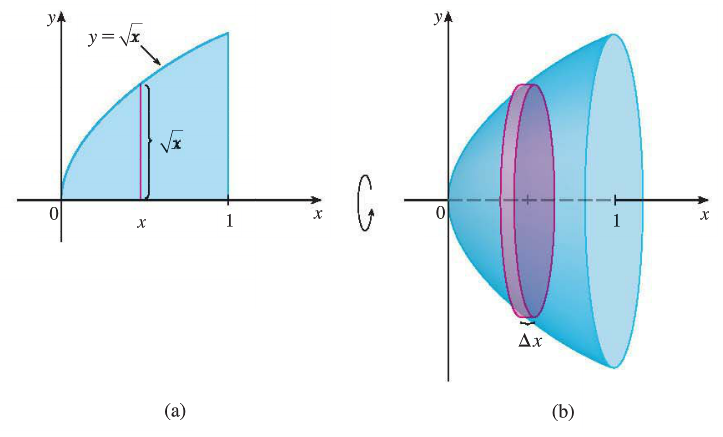
\includegraphics[scale=0.38]{6-2pic3.png}\]
  
  
  \vspace{2in}
  
  
  \underline{Example 3}: Find the volume of the solid obtained by rotating the region bounded by $y=x^3$, $y=8$, and $x=0$ about the $y-$axis.
  
  \[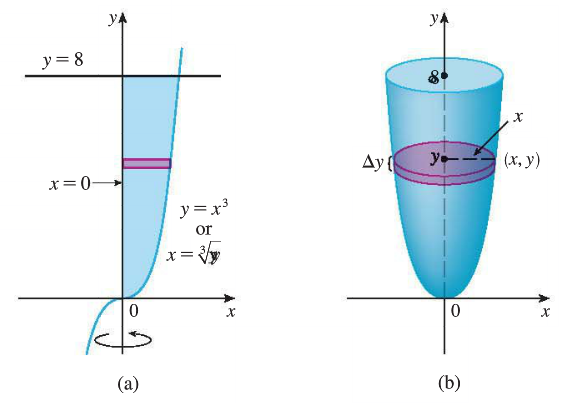
\includegraphics[scale=0.38]{6-2pic4.png}\]
  
  \vspace{2in}
  
  \section*{Washer Method}
 
 \underline{Example 4}: The region $\mathscr{R}$ enclosed by the curves $y=x$ and $y=x^2$ is rotated about the $x-$axis.
 \hphantom{Example 4 } Find the volume of the resulting solid.
 
 \[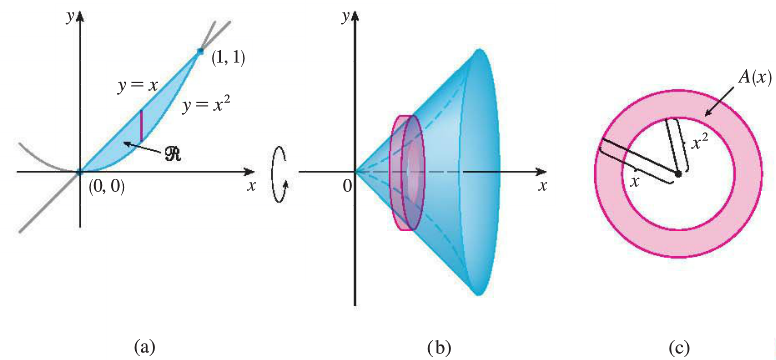
\includegraphics[scale=0.45]{6-2pic5.png}\]
 
Note: Here a cross section of the solid has the shape of a \underline{\hspace{1in}} with inner radius $x^2$ and outer radius $x$.\\
\indent

\vspace{2in}
  
 \underline{Example 5}: Find the volume of the solid obtained by rotating the region in Example 4 about the \hphantom{Example 5 } line $y=2$.\\
 
 
 \vspace{2.5in}
  \newpage
 \section*{Disk/Washer Method}
 
 The solids in Examples 1-5 are all called \textbf{solids of revolution} because they are obtained by revolving a region about a line. In general, we calculate the volume of a solid of revolution by using the basic defining formula:
 
 \[\underline{\hspace{2in}} \quad \quad \text{ or } \quad \quad \underline{\hspace{2in}}\]
 
 and we find the cross-sectional area $A(x)$ or $A(y)$ in one of the following ways:
 
 \begin{itemize}
 \item If the cross-section is a \underline{\hspace{0.75in}} (as in Examples 1-3), we find the radius of the disk (in terms of $x$ or $y$) and use
 \[A = \underline{\hspace{1.5in}}\]\\
 \item If the cross-section is a \underline{\hspace{1in}} (as in Examples 4-5), we find the inner radius $r$ and outer radius $R$ from a sketch and compute the area of the washer by subtracting the area of the inner disk from the area of the outer disk.
 
 \[A = \underline{\hspace{2.5in}} = \underline{\hspace{1.25in}}\]
 \end{itemize}

 \underline{Example 6}: Find the volume of the solid obtained by rotating the region in Example 4 about the line $x=-1$.\\
 \indent\\
 \indent
 
 
 
 \hspace{1in} 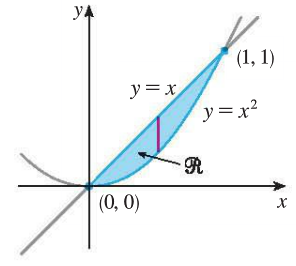
\includegraphics[scale=0.4]{6-2pic8.png}
 
 \vspace{2.5in}
 
 \newpage
 
 \section*{Volumes that are NOT solids of revolution}
 
 \underline{Example 7}: The figure below shows a solid with a circular base of radius 1. Parallel cross-sections perpendicular to the base are equilateral triangles. Find the volume of the solid. 
 
 \[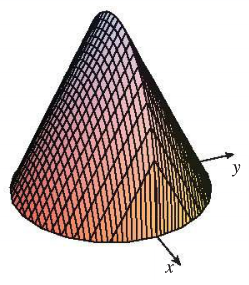
\includegraphics[scale=0.45]{6-2pic6.png} \quad 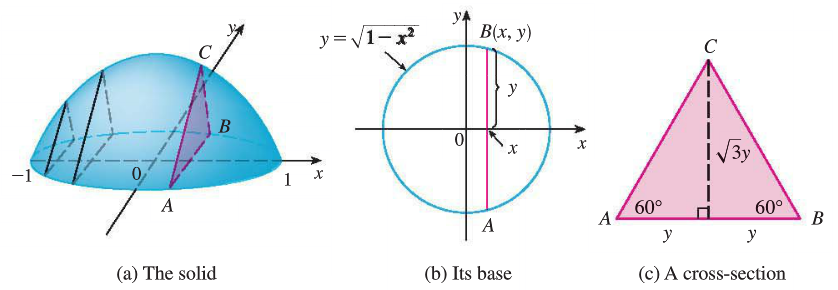
\includegraphics[scale=0.45]{6-2pic7.png}\]
 
 \vspace{3in}
 
 \newpage
 
 \underline{Example 8}: Find the volume of a pyramid whose base is a square with side $L$ and whose \hphantom{Example 8 } height is $h$.\\
 \indent
 
 
  \vspace{3.5in}

%----------------------------------------------------------------------------------------

\end{document}